% !TeX spellcheck = en_US
\section{Problem 7}
\subsection{Question A}
Let an activation function be
\begin{equation}
S(x) = \left\{
\begin{array}{cc}
	x^k, & x>L\\[1mm]
	x^k \dfrac{\left(L+x\right)^m}{\left(L+x\right)^m + \left(L-x\right)^m}, & \left|x\right| \le L\\[1mm]
	0, & x < -L
\end{array}
\right.
\end{equation}
This function has some parameters $k,L,m$ called hyperparameters. Using them, this function can approximate others.

\subsubsection{Swish}
%Swish: $k=1, \ L=2e, \ m=e$\\
In order for our activation function to approximate Swish, we have to see the latter first.
Swish's function is 
\[
S(x) = \dfrac{x}{1+e^{-x}} = x\dfrac{e^x}{1+e^x}
\]
and is plotted in figure~\ref{fig:prob7_swish}. In order to determine the parameters, we have to take a look in the plotted function. When $x>0$, Swish seems to be almost $y=x$, thus $k=1$. If we look at $x<0$, we can se that Swish curves until it settles back to 0.
That point $x_1$ where $Swish (x_1) = 0$ is parameter $L$. After trying multiple values, we opted with $2e$ as this gives the smaller overall error in that region.
After filling $k,L$, only parameter $m$ is left to be found. In general, $x^e$ is a good approximation of $e^x$, but an approximation only. Just trying $m=e$ and plotting the created function gets us the plot in figure~\ref{fig:prob7_swish} which is really close to Swish.
Finally, the activation function can be written 
\[
S(x) = \left\{
\begin{array}{cc}
	x, & x>2e\\[1mm]
	x \dfrac{\left(2e+x\right)^e}{\left(2e+x\right)^e + \left(2e-x\right)^e}, & \left|x\right| \le 2e\\[1mm]
	0, & x < -2e
\end{array}
\right.
\]

\begin{figure}[H]
	\centering
	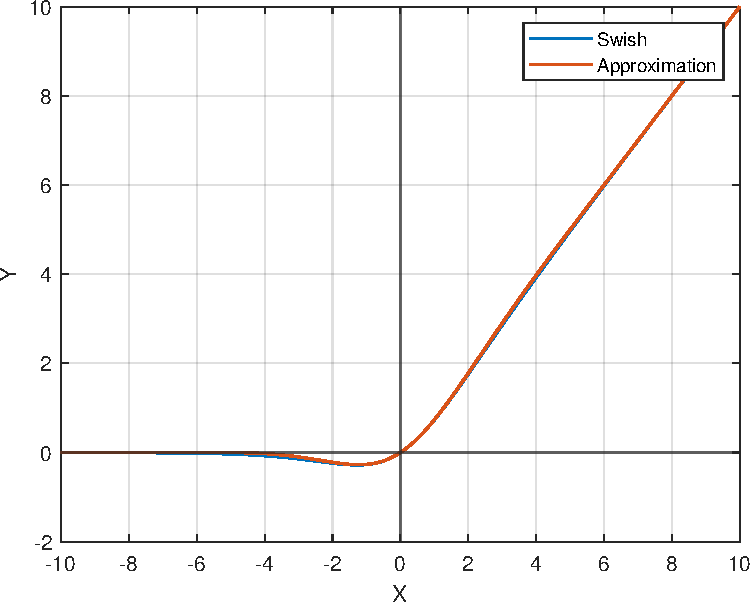
\includegraphics[width=.5\textwidth]{../Problem 7/prob7_swish.pdf}
	\caption{Swish activation function and its approximation.}
	\label{fig:prob7_swish}
\end{figure}

\subsubsection{Sigmoid}
Sigmoid's function is 
\[
S(x) = \dfrac{1}{1+e^{-x}} = \dfrac{e^x}{1+e^x}
\]
Just from this type, we understand that is $\frac{Swish(x)}{x}$. So, selecting parameters is easier this time as $m$ and $L$ will not change. Because of the previous equation, parameter $k$ must be decreased by $1$, thus $k=0$. Figure~\ref{fig:prob7_sigmoid} shows both the sigmoid and its approximation.

\begin{figure}[H]
	\centering
	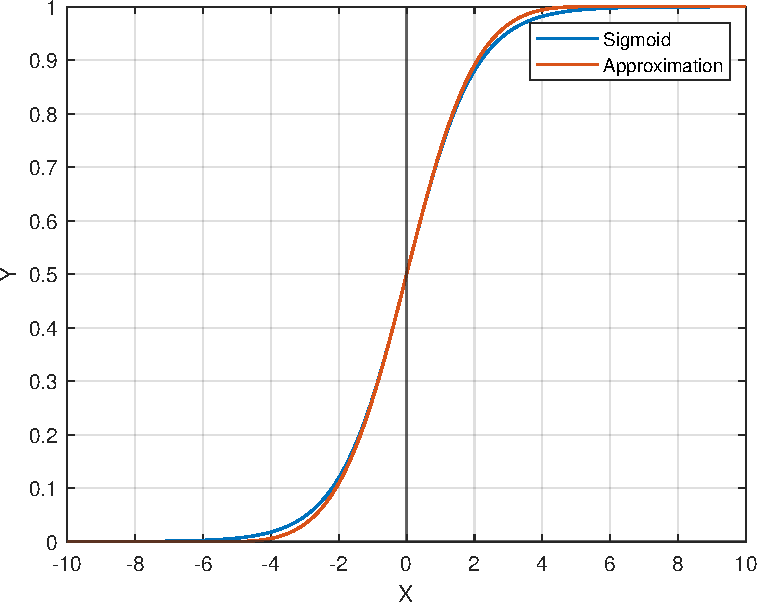
\includegraphics[width=.5\textwidth]{../Problem 7/prob7_sigmoid.pdf}
	\caption{Sigmoid activation function and its approximation.}
	\label{fig:prob7_sigmoid}
\end{figure}


\subsubsection{ReLU}
ReLU is defined as 
\[
ReLU(x) = \max(0,x) = \left\{
\begin{array}{cc}
	0, & x<0\\
	x, & x \ge 0
\end{array}
\right.
\]
From this, we can already determine parameter $k$ to be $k=1$, as we want $x^k = x \Rightarrow k=1$.
Setting $L=0$ ensures that the transition point between the linear and non-linear parts of the function occurs at $x=0$, which is consistent with the behavior of ReLU.
Also, setting $m=0$ means that the denominator term becomes $1$ for both the linear and non-linear parts of the function, simplifying the expression.
The plotted functions are presented in figure~\ref{fig:prob7_relu}\\
With parameters those mentioned above, $S(x)$ is the following
\[
S(x) = \left\{
\begin{array}{cc}
	x, & x\ge 0\\
	0, & x < 0
\end{array}
\right.
\]

\begin{figure}[H]
	\centering
	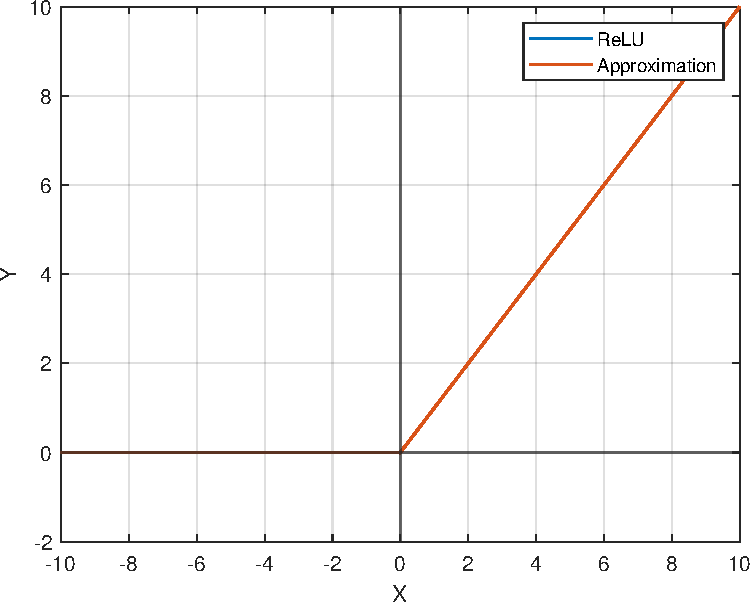
\includegraphics[width=0.5\textwidth]{../Problem 7/prob7_relu.pdf}
	\caption{ReLU activation function and its approximation.}
	\label{fig:prob7_relu}
\end{figure}


\subsection{Question B}

\subsubsection{Derivative with respect to x}
\[
\begin{gathered}
\dfrac{dS}{dx} = kx^{k-1} + x^k\dfrac{m\left(L+x\right)^m \left(\left(L+x\right)^{m-1} + \left(L-x\right)^{m-1}\right) - \left(L+x\right)^m \left( m\left(L+x\right)^{m-1}  + m\left(L-x\right)^{m-1}\right)}{\left( \left(L+x\right)^m + \left(L-x\right)^m \right)^2}=\\[1mm]
= kx^{k-1}
\end{gathered}
\]

\subsubsection{Derivative with respect to k}
We know from algebra that $\dfrac{d}{dx}\left(a^x\right) = a^x \ln a$. So
\[
\dfrac{dS}{dk} = x^k \ln (k) \dfrac{\left(L+x\right)^m}{\left(L+x\right)^m + \left(L-x\right)^m} 
\]

\subsubsection{Derivative with respect to L}
\[

\]